\documentclass{article}
% Change "article" to "report" to get rid of page number on title page
\usepackage{amsmath,amsfonts,amsthm,amssymb}
\usepackage{setspace}
\usepackage{Tabbing}
\usepackage{fancyhdr}
\usepackage{lastpage}
\usepackage{extramarks}
\usepackage{url}
\usepackage{chngpage}
\usepackage{longtable}
\usepackage{soul,color}
\usepackage{graphicx,float,wrapfig}
\usepackage{enumitem}
\usepackage{morefloats}
\usepackage{multirow}
\usepackage{multicol}
\usepackage{indentfirst}
\usepackage{lscape}
\usepackage{pdflscape}
\usepackage{natbib}
\usepackage[toc,page]{appendix}
\providecommand{\e}[1]{\ensuremath{\times 10^{#1} \times}}

% In case you need to adjust margins:
\topmargin=-0.45in      % used for overleaf
%\topmargin=0.25in      % used for mac
\evensidemargin=0in     %
\oddsidemargin=0in      %
\textwidth=6.5in        %
%\textheight=9.75in       % used for mac
\textheight=9.25in       % used for overleaf
\headsep=0.25in         %

% Homework Specific Information
\newcommand{\hmwkTitle}{Progress Report 1}
\newcommand{\hmwkDueDate}{Monday,\ September\  24,\ 2018}
\newcommand{\hmwkClass}{Final Project}
\newcommand{\hmwkClassTime}{CSE 597}
\newcommand{\hmwkAuthorName}{Wenliang\ Sun}
\newcommand{\hmwkNames}{wzs51}

% Setup the header and footer
\pagestyle{fancy}
\lhead{\hmwkNames}
\rhead{\hmwkClassTime: \hmwkTitle} 
\cfoot{Page\ \thepage\ of\ \pageref{LastPage}}
\renewcommand\headrulewidth{0.4pt}
\renewcommand\footrulewidth{0.4pt}

%%%%%%%%%%%%%%%%%%%%%%%%%%%%%%%%%%%%%%%%%%%%%%%%%%%%%%%%%%%%%
% Make title

\title{\vspace{2in}\textmd{\textbf{\hmwkClass:\ \hmwkTitle}} \\
\vspace{0.1in}\large{ \hmwkClassTime}\vspace{3in}}

\author{\textbf{\hmwkAuthorName} \\ \vspace{0.1in}
\hmwkDueDate }
\date{} % to take away today's date

%%%%%%%%%%%%%%%%%%%%%%%%%%%%%%%%%%%%%%%%%%%%%%%%%%%%%%%%%%%%%

\begin{document}
\begin{spacing}{1.1}
\maketitle

\newpage
\section*{Abstract}

The convection-diffusion equation is a combination of the diffusion and convection equations, and describes physical phenomena where particles, energy, or other physical quantities are transferred inside a physical system due to two processes: diffusion and convection. Depending on context, the same equation can be called the advection–diffusion equation, drift–diffusion equation, or scalar transport equation.

In this project, we leverage a program to solve a 2D convection-diffusion equation. We have two different solvers: direct solver and iterative solver. We use LU decomposition and Jacobi methods to implement our project. After that, we compare their performance. 

\section{Problem of Interest}

\begin{itemize}
    As we learn in class, the problem is to solve partial differential equation.
    In my project, I am going to solve a 2D convection-diffusion problem. As a very important branch of partial differential equations, convection-diffusion equations have been widely used in many fields, such as fluid mechanics, gas dynamics, etc. Because convective diffusion equations are difficult to obtain analytical solutions through analytical methods, so through various numerical methods to solve the convection-diffusion equation plays an important role in numerical analysis. My project solves the steady 2D convection-diffusion problem: 
    $\frac{\partial \rho u_i \phi}{\partial x_i}$ = $\frac{\partial (\tau \frac{\partial \phi }{\partial x_i})}{\partial x_i}$ + $q_\phi$. 

\end{itemize}

\subsection{Numerical Set-up}

\begin{itemize}

    For the 2D convection diffusion equation, we assume: \newline\newline
    
    x$\in$[0,1] and y$  \in$[0,1] and $\rho$ = 100, $\tau$ = 0.1, $q_\phi$ = 0, $u_x=x$, and $u_y=-y$. The boundary conditions are $\phi$=0 on y = 1, $\phi$ = $\phi$(y) = 1-y on x=0, $\frac{\partial \phi}{\partial x}$ = 0 on x = 1, and $\frac{\partial \phi}{\partial y}$ on y = 0. \newline\newline
    
    According the above conditions, we can discretize the problem. We use a small size matrix as an simple example. And then divide the area into a 5*5 matrix as figure 1.\newline\newline
    
    \begin{figure}[H]
    \centering
    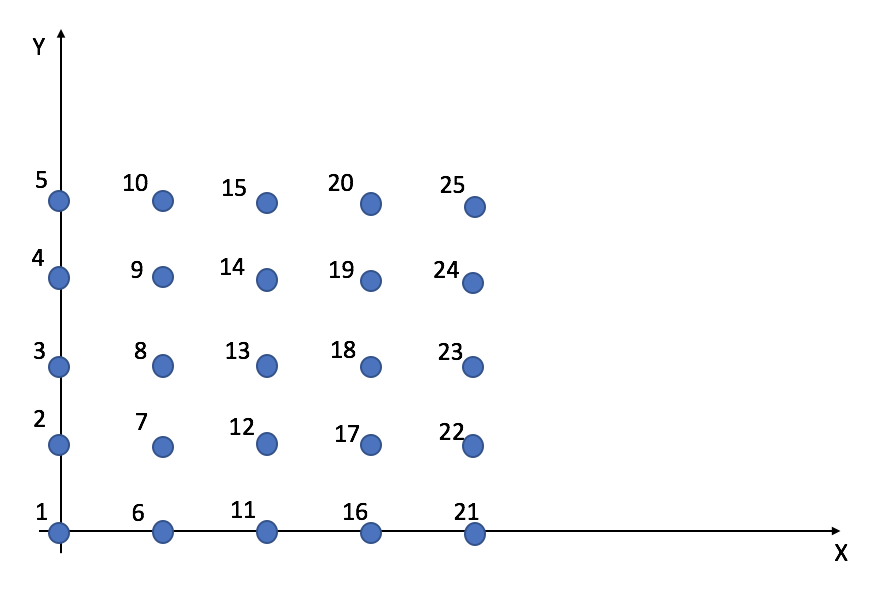
\includegraphics[width=8.0cm]{figure1.png}
    \caption{This is an example of a 5*5 matrix}
    \label{figure 1.1}
    \end{figure}

    
    \begin{figure}[H]
    \centering
    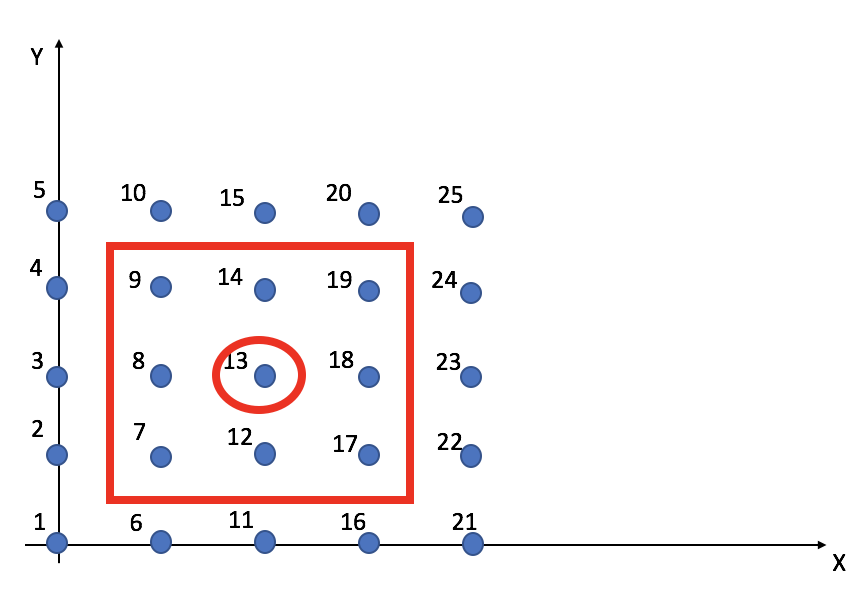
\includegraphics[width=8.0cm]{figure2.png}
    \caption{This is an example of an interior node}
    \label{figure 2}
    \end{figure}
    
    Firstly, we calculate the interior nodes. In the figure 2, the interior nodes are in the red circle. We use node 13 as an example. The other interior nodes' calculation are same. For the node 13, we leverage the Second-order Central Difference Scheme(CDS2) to solve it. According to the node 8, 18, 12, 14, we can get: \newline\newline
    $(\rho u_x/2h - \tau / h^2)\phi_{18}  + (-\rho u_x/2h - \tau / h^2)\phi_8 + 4 \tau/h^2 \phi_{13} + (\rho u_y/2h - \tau / h^2)\phi_{14}  + (-\rho u_y/2h - \tau / h^2)\phi_{12} = q_\phi$  \newline\newline

    In this equation, "h" stand for the distance between two nodes. Through this method, we can calculate all the interior nodes. And we can use the coefficients to build A matrix. There are nine interior nodes, so it could fill in nine lines in A matrix, and the same position of b matrix is "0". \newline
    
    Secondly, we should solve the boundary problem. For this example, there are four boundaries: left, right, up and down. The left boundary is a constant, it is "1-y". So we can fill in the A matrix with "0", and set the node's position in A matrix as "1". The corresponding position in b matrix is "1-y". The up boundary is similar as the left boundary, the difference is that the corresponding position in b matrix is "0".\newline 
    
    But the right boundary is different, they are Newman Boundary Condition. We use Second-order Backward Difference Scheme(BDS2) to solve it. This method means that we use the two nodes behind it. We use node 23 as an example. We can get the equation:\newline\newline
    \centerline{$\frac{\phi_13 - 4 \phi _{18} + 3\phi_{23} }{2\Delta x} = f(y)|_{23}$}\newline\newline
    Because the $\frac{\partial \phi}{\partial x}$ = 0 on x = 1, so we can get: 
    ${\phi_{13} - 4 \phi _{18} + 3\phi_{23}}$=0. And then we fill in A matrix with these coefficients. And the corresponding position of b matrix is "0". \newline
    
    In the end, we can generate the A matrix and b matrix by merging the two parts as above. 
    
\end{itemize}

\section{Solvers}

\subsection{Direct Solver}

\begin{itemize}

    In my project, I choose LU decomposition solver as the direct approach. As we learned in class, this type of solver decompose A matrix into L and U matrix. In the real world, there may be lots of calculations to solve the whole problem. So the matrix decomposition method is much more convenient than other methods such as Gauss elimination.\newline
    According our experiment, for a 25 * 25 nodes matrix, the memory allocated for the test case is about 3 MB for saving the matrices L and U, and about another 1.5 MB to save the original matrix A. But in my example, the A matrix is just 25*25, so it is only occupy a small size of memory. And it is very fast to run the example case. I will generate bigger data size in my future works.
\end{itemize}

\subsection{Iterative Solver}

\begin{itemize}
   
    I use Jacobi method as iterative solver in our project. According to the Dr. Adam's code, we implement our Jacobi solver. Generally speaking, the Jacobi solver is based on the convergence. It also could be used in the future parallel implementations. In my test case, the two solvers seems like have similar time consumption. But according to the algorithm complexity, the iterative solver must be better than the direct solver when the problem scale is huge. For the memory problem, because my the scale of problem is small, so it just costs several kilobytes.
\end{itemize}

\section{Solver Comparison}

\begin{itemize}
    According to our experiments, we find that the direct method is very practical in general problems when the dimension is small (the rank of the coefficient matrix is less than 100). The convergence of iterative methods varies widely among different problems. Jacobi iterative method are used to solve large sparse matrices. However, its convergence is difficult to guarantee.\newline
    For the production problems, the direct solver is limited by the algorithm complexity. Therefore before the memory exhausts, it is very likely that the computation time becomes unacceptable. For the iterative solver, the most vital element is iteration numbers, for the memory consumption is of the same order of magnitude of the consumption for saving an input field. To implement these solvers parallel, our codes must run on many cores. Therefore the functions should be modified in the future work.
\end{itemize}

\section{Discussion and Conclusions}

\begin{enumerate}
    In this project, we describe the basic idea of the 2D convection-diffusion equation, and then solve the equation by direct solver and iterative solver. We also have discussed the method of discretization, the construction of A matrix and b matrix and the comparison of these two methods.\newline
    But there are also some limitations. The first one is the matrix is not big enough. It makes the results are not obvious. And the second one is the code is not "smart". Some input data and parameters we fix them in the codes. It is not easy to modify them. The last one is my Jacobi function. There are small bugs. If the input is too big, such as a 625*625 matrix, the result is not accuracy. These problems we will optimize in our future work.  
\end{enumerate}

\newpage
\begin{appendices}

\section{Acknowledgements}
My mathematics and C abilities are not very well. The last time I solved PDE was about 6 years ago. And I use Java several years, my program are translated from Java to C. So this project would not have been possible without the support of Dr. Adam Lavely, Dr. Christopher Blanton and my classmate Yueze Tan. I am especially indebted to my friends Tianyuan Wei and Xingzhao Yun. Tianyuan Wei is an Earth and Mineral Science student, he gave me his class notes and taught me how to solve the PDE step by step; Xingzhao Yun is good at C and CPP, he taught me the basic syntax. They worked actively to provide me the help to complete the Ax = b problem.

\section{Code}

\begin{itemize}
    \item LU.cpp: Using LU method to solve the equations. According to the comments, modify the input before you use it.
    \item Jacobi.cpp: Using Jacobi method to solve the equations. According to the comments, modify the input before you use it.
    \item GetMatrix.cpp: Using this class to generate matrix A and b. According to the comments, modify the input before you use it.
    \item We use PSU ACI run the codes.
    
    All files are on our github, the address is https://github.com/William0617/CSE597HW1.
    These above files can be compiled by the command "gcc filename.cpp -o filename". And all the output will be showed on the terminal.
\end{itemize}

\section{Licensing and Publishing}

\begin{itemize}
    The GNU license is used in this project. The detailed information could be seen in the license.txt and gpl.txt in the root folder of this project.\newline
    And the report is published in CSE 597 course, the Pennsylvania State University. 
\end{itemize}
\end{appendices}





\bibliographystyle{acm}
\bibliography{progressReport}

\end{spacing}

\end{document}

%%%%%%%%%%%%%%%%%%%%%%%%%%%%%%%%%%%%%%%%%%%%%%%%%%%%%%%%%%%%%}}
